
%----------------------------------------------------------------------------------------
%	Machine Learning Assignment Template
%----------------------------------------------------------------------------------------

\documentclass[11pt]{scrartcl}
\newcommand*\student[1]{\newcommand{\thestudent}{{#1}}}

%----------------------------------------------------------------------------------------
%	INSERT HERE YOUR NAME
%----------------------------------------------------------------------------------------

\student{Omenetti Matteo, Srinivasan Ravi}

%----------------------------------------------------------------------------------------
%	PACKAGES AND OTHER DOCUMENT CONFIGURATIONS
%----------------------------------------------------------------------------------------

\usepackage[utf8]{inputenc} % Required for inputting international characters
\usepackage[T1]{fontenc} % Use 8-bit encoding
\usepackage[sc]{mathpazo}
\usepackage{caption}
\usepackage{subcaption}
\usepackage{hyperref}
\usepackage{inconsolata}

\usepackage[english]{babel} % English language hyphenation
\usepackage{amsmath, amsfonts} % Math packages
\usepackage{listings} % Code listings, with syntax highlighting
\usepackage{graphicx} % Required for inserting images
\graphicspath{{Figures/}{./}} % Specifies where to look for included images (trailing slash required)
\usepackage{float}
\usepackage{mathtools}
\usepackage{booktabs}


%----------------------------------------------------------------------------------------
%	DOCUMENT MARGINS
%----------------------------------------------------------------------------------------

\usepackage{geometry} % For page dimensions and margins
\geometry{
	paper=a4paper, 
	top=2.5cm, % Top margin
	bottom=3cm, % Bottom margin
	left=3cm, % Left margin
	right=3cm, % Right margin
}

%----------------------------------------------------------------------------------------
%	SECTION TITLES
%----------------------------------------------------------------------------------------

\usepackage{sectsty}
%\sectionfont{\vspace{6pt}\centering\normalfont\scshape}
\subsectionfont{\normalfont\bfseries} % \subsection{} styling
\subsubsectionfont{\normalfont\itshape} % \subsubsection{} styling
\paragraphfont{\normalfont\scshape} % \paragraph{} styling

%----------------------------------------------------------------------------------------
%	HEADERS AND FOOTERS
%----------------------------------------------------------------------------------------

\usepackage{scrlayer-scrpage}
\ofoot*{\pagemark} % Right footer
\ifoot*{\thestudent} % Left footer
\cfoot*{} % Centre footer

%----------------------------------------------------------------------------------------
%	TITLE SECTION
%----------------------------------------------------------------------------------------

\title{	
	\normalfont\normalsize
	\textsc{Machine Learning for Health Care\\%
	ETH Zürich}\\
	\vspace{25pt}
	\rule{\linewidth}{0.5pt}\\
	\vspace{20pt}
	{\huge Project 1}\\
	\vspace{12pt}
	\rule{\linewidth}{1pt}\\
	\vspace{12pt}
}

\author{\LARGE \thestudent}

\date{\normalsize\today}

\begin{document}

\maketitle
\newpage
\tableofcontents
\newpage



\section{Introduction}
This report is part of the first project for the course "Machine Learning for Health Care" hosted at ETH Zürich. The scope of this project was to build different models for ECG classification for two different datasets PTB and MIT\_BIH.  All of the models described in this report can be found in  "src/" and they have been trained (in a reasonable amount of time) using the GPUs/TPUs offered by Google COLAB-Pro. All of the images that summarize the achitecture of the different models have been omitted due to the length constraints of the report, but can be found in the respective notebooks together the graphs for the training loss and accuracy and the confusion matrices for multiclass classification.


%%%%%%%%%%%%%%%%%%%%%%%%%%%%%%%%%%%%% VANILLA CNN %%%%%%%%%%%%%%%%%%%%%%%%%%%%%%%%%%%%%%%%%%%%%%%%%%
\section{Convolutional Neural Network (CNN)}
For the vanilla CNN, a smaller model compared to the one provided as a baseline was built. The reason behind this shallower architecture is that we were curious to understand whether the decreased training cost would also result in a statistically relevant decrease in performance. However, as it will be reported in the two subsections below this is not the case. 

%%%%%%% MIT %%%%%%%
\subsection{MIT\_BIH}
The model on the Mit\_Bih dataset achieves a test accuracy score of 0.982, taking around 6 minutes to train. This model was trained for 25 epochs with the option to reduce the learning rate on plateau, early stopping and validaiton split 0.1.
The reported accuracy show the performance of this shallower model are very close to the baseline model (accuracy 0.985)  that instead takes more than 7 minutes to train on the same GPU.

%%%%%%% PTB %%%%%%%
\subsection{PTB}
The model on the PTB dataset achieves a test accuracy score of 0.975, taking around 1 minute to train. This model was trained for 33 epochs with the option to reduce the learning rate on plateau, early stopping and validation split 0.1.
The reported accuracy show, the performance of this shallower model is very close to the baseline model (accuracy 0.991). The model achieved a AUROC score of 0.974 and a AUPRC score of 0.983.

%%%%%%%%%%%%%%%%%%%%%%%%%%%%%%%%%%%%% VANILLA RNN %%%%%%%%%%%%%%%%%%%%%%%%%%%%%%%%%%%%%%%%%%%%%%%%%%
\section{Recurrent Neural Network (RNN)}
This model consists of three sequential SimpleRNN blocks (respectively with dimension 128, 256 and 100), followed by a dense layer to perform the classification. The model is trained by unrolling the RNN blocks to speed up the training with GPUs.
%%%%%%% MIT %%%%%%%
\subsection{MIT\_BIH}
The training completed in 40 epochs (40s/epochs) with early stopping and validation split set at 0.2.
This model on the Mit\_Bih dataset achives an accuracy of 0.888. 

%%%%%%% PTB %%%%%%%
\subsection{PTB}
 The training completed in 89 epochs (5s/epochs) with early stopping and validation split set at 0.2.
This model on the Mit\_Bih dataset achives an accuracy of 0.795. The model achieved a AUROC score of 0.857 and a AUPRC score of 0.940.

%%%%%%%%%%%%%%%%%%%%%%%%%%%%%%%%%%%%%  DBLSTM-WS %%%%%%%%%%%%%%%%%%%%%%%%%%%%%%%%%%%%%%%%%%%%%%%%%%
\section{DBLSTM-WS}
This network consists of 2 Bidirectional LSTM blocks (dimension 128 and 64) both with return\_sequences=True and dropout rate at 0.01. A dense layer follows with dimension 128 and dropout rate 0.3 and ReLu as actiavtion function. A final dense layer follows for classification. The network takes as input a matrix where the first layer represents the original signal, while the other rows each represent the DWT (discrete wavelet decomposition) of the previous row. To achieve this we use the pywavelet library and the Daubechies db6 wavelet member (the rows are padded to 0 to obtain same-length signals). In both cases we found that using 3 levels of discrete wavelet transforms.
%%%%%%% MIT %%%%%%%
\subsection{MIT\_BIH}
The model trained for 25 epochs (22sec/epochs) using early stopping, reduce LR on plateau and validation split 0.2.
This model on the Mit\_Bih dataset achives an accuracy of 0.985.

%%%%%%% PTB %%%%%%%
\subsection{PTB}
The model trained for 41 epochs (2sec/epochs) using early stopping, reduce LR on plateau and validation split 0.2.
This model on the PTB dataset achives an accuracy of 0.986. The model achieved a AUROC score of 0.995 and a AUPRC score of 0.997.

%%%%%%%%%%%%%%%%%%%%%%%%%%%%%%%%%%%%% RES NET %%%%%%%%%%%%%%%%%%%%%%%%%%%%%%%%%%%%%%%%%%%%%%%%%%
\section{CNN with Residual Blocks}
For this task, we designed a CNN architecture similar to ResNet (but shallower). This is the model that achieves the best performance. This model compared to the vanilla CNN adds residual blocks after each BatchNormalization layer.
%%%%%%% MIT %%%%%%%
\subsection{MIT\_BIH}
The model trained for 27 epochs (15sec/epochs) using early stopping, reduce LR on plateau and validation split 0.1.
This model on the Mit\_Bih dataset achives an accuracy of 0.988.

%%%%%%% PTB %%%%%%%
\subsection{PTB}
The model trained for 44 epochs (2sec/epochs) using early stopping, reduce LR on plateau and validation split 0.1.
This model on the PTB dataset achives an accuracy of 0.986. The model achieved a AUROC score of 0.857 and a AUPRC score of 0.94

%%%%%%%%%%%%%%%%%%%%%%%%%%%%%%%%%%%%% TRANSFORMER %%%%%%%%%%%%%%%%%%%%%%%%%%%%%%%%%%%%%%%%%%%%%%%%%%
\section{Transformer}
This model consists of three transformers encoder blocks, stacked on top of each other with a standard CNN at the end. This model is very heavy to train. Without ColabPro the training for the Mit\_Bih dataset is around 16hours with the TPU.  Using ColabPro, the amount of time required to train the model decreases drastically. Overall, its performance is not great if compared to the other much lighter models, therefore we would not recommend using this model in these particular tasks. Moreover, this model is also significantly slower than all of the other models at prediction time.
%%%%%%% MIT %%%%%%%
\subsection{MIT\_BIH}
The model trained for 104 epochs (25sec/epochs) using early stopping and validation split 0.2.
This model on the Mit\_Bih dataset achives an accuracy of 0.976. 

\begin{figure}[H]
	\centering
	\begin{subfigure}{.30\textwidth}
		\centering
		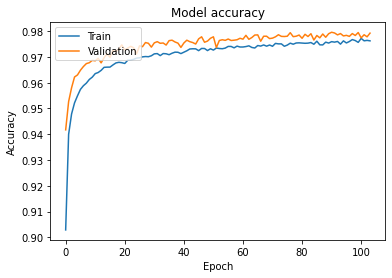
\includegraphics[width=.95\linewidth]{../models_performance_graphs/mit/transformer_mit_accuracy.png}  
		\caption{Train and validation loss of the transformer for the Mit\_bih dataset.}
	\end{subfigure}
	\begin{subfigure}{.30\textwidth}
		\centering
		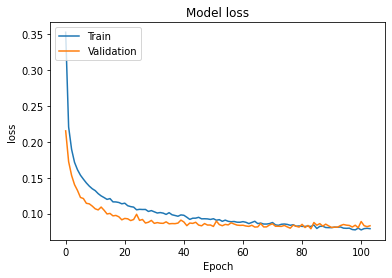
\includegraphics[width=.95\linewidth]{../models_performance_graphs/mit/transformer_mit_loss.png}  
		\caption{Train and validation accuracy of the transformer for the Mit\_bih dataset.}
	\end{subfigure}
	\begin{subfigure}{.30\textwidth}
		\centering
		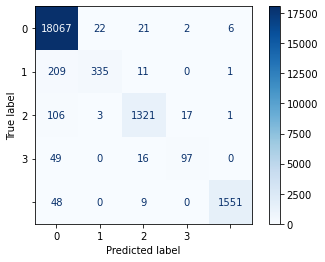
\includegraphics[width=.95\linewidth]{../models_performance_graphs/mit/transformer_mit_confusion.png}  
		\caption{Confusion matrix of the transformer for the Mit\_bih dataset.}
	\end{subfigure}
	\label{FIGURE LABEL 1}
	\caption{}
\end{figure}

%%%%%%% PTB %%%%%%%
\subsection{PTB}
The model trained for 146 epochs (4sec/epochs) using early stopping and validation split 0.2.
This model on the PTB dataset achives an accuracy of 0.968. The model achieved a AUROC score of 0.980 and a AUPRC score of 0.985.

%%%%%%%%%%%%%%%%%%%%%%%%%%%%%%%%%%%%% Transfer Learning %%%%%%%%%%%%%%%%%%%%%%%%%%%%%%%%%%%%%%%%%%%%%%%%%%
\section{Transfer Learning}
For this task we used the DBLSTM-WS model trained on the MIT\_BIH dataset. We froze the Bidirectional LSTM layers and then trained the last two dense layers on the PTB dataset (adapting the last layer to fit the binary classification task), thus making these layers perform feature extraction. The model trained for 27 epochs (3sec/epoch) using early stopping, reduce LR on plateau and validation split 0.2.
This model on the PTB dataset achives an accuracy of 0.992. The model achieved a AUROC score of 0.996 and a AUPRC score of 0.997. We also tried to freeze the first dense layer and only train the last dense obtaining an accuracy of 0.988.

\begin{figure}[H]
	\centering
	\begin{subfigure}{.47\textwidth}
		\centering
		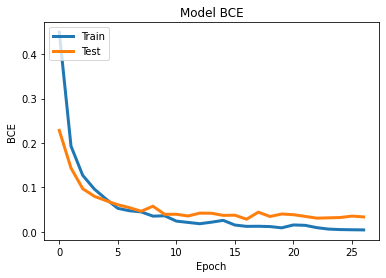
\includegraphics[width=.95\linewidth]{../models_performance_graphs/ptb/transf_ptb_accuracy.png}  
		\caption{Train and validation loss of the transfer learning for the PTB dataset.}
	\end{subfigure}
	\begin{subfigure}{.47\textwidth}
		\centering
		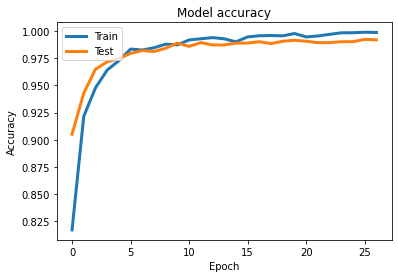
\includegraphics[width=.95\linewidth]{../models_performance_graphs/ptb/transf_ptb_loss.png}  
		\caption{Train and validation accuracy of the transformer for the PTB dataset.}
	\end{subfigure}
	\label{FIGURE LABEL 2}
	\caption{}
\end{figure}


%%%%%%%%%%%%%%%%%%%%%%%%%%%%%%%%%%%%% ENSEMBLE %%%%%%%%%%%%%%%%%%%%%%%%%%%%%%%%%%%%%%%%%%%%%%%%%%
\section{Ensemble of models}
For this optional ensemble task, we decided to use two different approaches. For the first approach, we just summed up the different prediction probabilities of every model, and then we took the class with the highest one. For the second approach, we ran a logistic regression model on the output probabilities of every model, in order to better understand the relation between the models. 
The logistic regression ensemble achieves the best performance among all the models used for this assignment with an accuracy for the PTB dataset of 99.1\%. Once again ensembles of models of different kinds prove to be more robust than each single model taken separately.
The performance of each approach is summarized in their respective section.

%%%%%%% ENSEMBLE ONE %%%%%%%
\subsection{Average of the outputs}
%%%%%%% MIT %%%%%%%
\subsubsection{MIT\_BIH}
This ensemble reaches an accuracy of 0.984.

%%%%%%% PTB %%%%%%%
\subsubsection{PTB}
This ensemble reaches an accuracy of 0.990. The model achieved a AUROC score of 0.986 and a AUPRC score of 0.990.

%%%%%%% ENSEMBLE TWO %%%%%%%
\subsection{Logistic regression on the outputs}

%%%%%%% MIT %%%%%%%

\subsubsection{MIT\_BIH}
This ensemble reaches an accuracy of 0.987.

%%%%%%% PTB %%%%%%%
\subsubsection{PTB}
This ensemble reaches an accuracy of 0.991. The model achieved a AUROC score of 0.988 and a AUPRC score of 0.991.

\newpage
\section{Appendix}

\begin{table}[ht]
\centering
\caption{Summary of results - Accuracy}
\begin{tabular}[t]{lcc}
\toprule
&MIT\_BIH A&PTB\\
\midrule
Vanilla CNN &0.981&0.982\\
Vanilla RNN & 0.888 & 0.795 \\
DBLSTM-WS & 0.985 & 0.986 \\
CNN Residual Blocks&0.988&0.986\\
Transformer&0.976&0.968\\
Transfer Learning & -- & 0.992 \\
Ensemble Average&0.984&0.990\\
Ensemble Logistic&0.987&0.991\\
\bottomrule
\end{tabular}
\end{table}

\end{document}
